\section{S-ENSO's impact on large-scale conditions over the Atlantic}
To propose possible physical pathways by which our index impact Atlantic TC activity, we compute the composites for factors known to influence Atlantic TC activity: potential intensity (PI), vertical wind shear between 850 and 200 hPa, and SST. Each composite was for the August-October period - the peak hurricane season. To compare how well our index resolves the large-scale conditions that are critical to seasonal TC activity we compare our index' composites to those of the seasonal TC count composites (baseline) and those of the most common warming-based ENSO index: NINO3.4. The idea is that if our index is better able to distinguish between the large-scale conditions for active and inactive hurricane seasons its composites should closely resemble those of the baseline (i.e. active minus inactive hurricane years). Furthermore, Recent hurricane downscaling studies \cite{knutson2007simulation, emanuel2010comparison} as well as genesis indices \cite{menkes2012comparison} have shown that the large scale environment over the Atlantic might play a dominant role in modulating Atlantic TC activity than precursor disturbances, since these simulations do not model such disturbances yet are able to reproduce Atlantic TC climatology with significant accuracy.

%Previous work investigating the ENSO-Atlantic TC teleconnection proposed that enhanced convection as a result of anomalous Pacific Ocean warming during the El Niño phase is associated with strong westerly upper tropospheric wind over the Caribbean basin and tropical Atlantic, resulting in low TC activity during ENSO's warm phase (El Ni\~{n}o) events and high TC activity during its cold phase (La Ni\~{n}a). Warm eastern Pacific SST and negative (drought) Sahelian rainfall anomalies are associated with suppressed Atlantic basin tropical cyclone activity through an equatorially confined near-zonal circulation with upper-level westerlies and lower-level easterlies that act to increase the climatological westerly vertical shear in the main development region \cite{goldenberg1996physical}. Other studies have suggested that ENSO impact Atlantic TC activity via tropospheric warming \cite{tang2004}, since warm free tropospheric temperatures that are spread eastward from the Pacific by equatorial wave dynamics (e.g. Kelvin waves) can inhibit TC activity by providing a too weak vertical temperature gradient for TC activity to occur. Analogous to reduced vertical temperature gradient, a reduced vertical gradient of saturation deficit suppresses vertical mixing and thus negatively affects TC activity.

However, it seems that by monitoring the deep convection associated with the region with the highest Pacific SST warming anomaly, we succeed to observe the strength and location of updrafts related to this convection and the resulting strength and location of the zonal Walker circulation, as well as its impact on the tropical Atlantic circulation, as described in e.g. \cite{liu2004remote}, who  suggest that the remote impact contributes to nearly half of the variance of the tropical Atlantic SST variability at interannual and decadal time scales. Updrafts over the eastern and central Pacific during El Ni\~no result in downdrafts and therefore reduced TC activity over the tropical Atlantic, whereas updrafts over the western Pacific during neutral and La Ni\~na years result in downdrafts over the eastern tropical Pacific and updrafts over the Atlantic, thus leading to increased TC activity.

\begin{figure}[htbp]

\hspace{-2.5cm}		
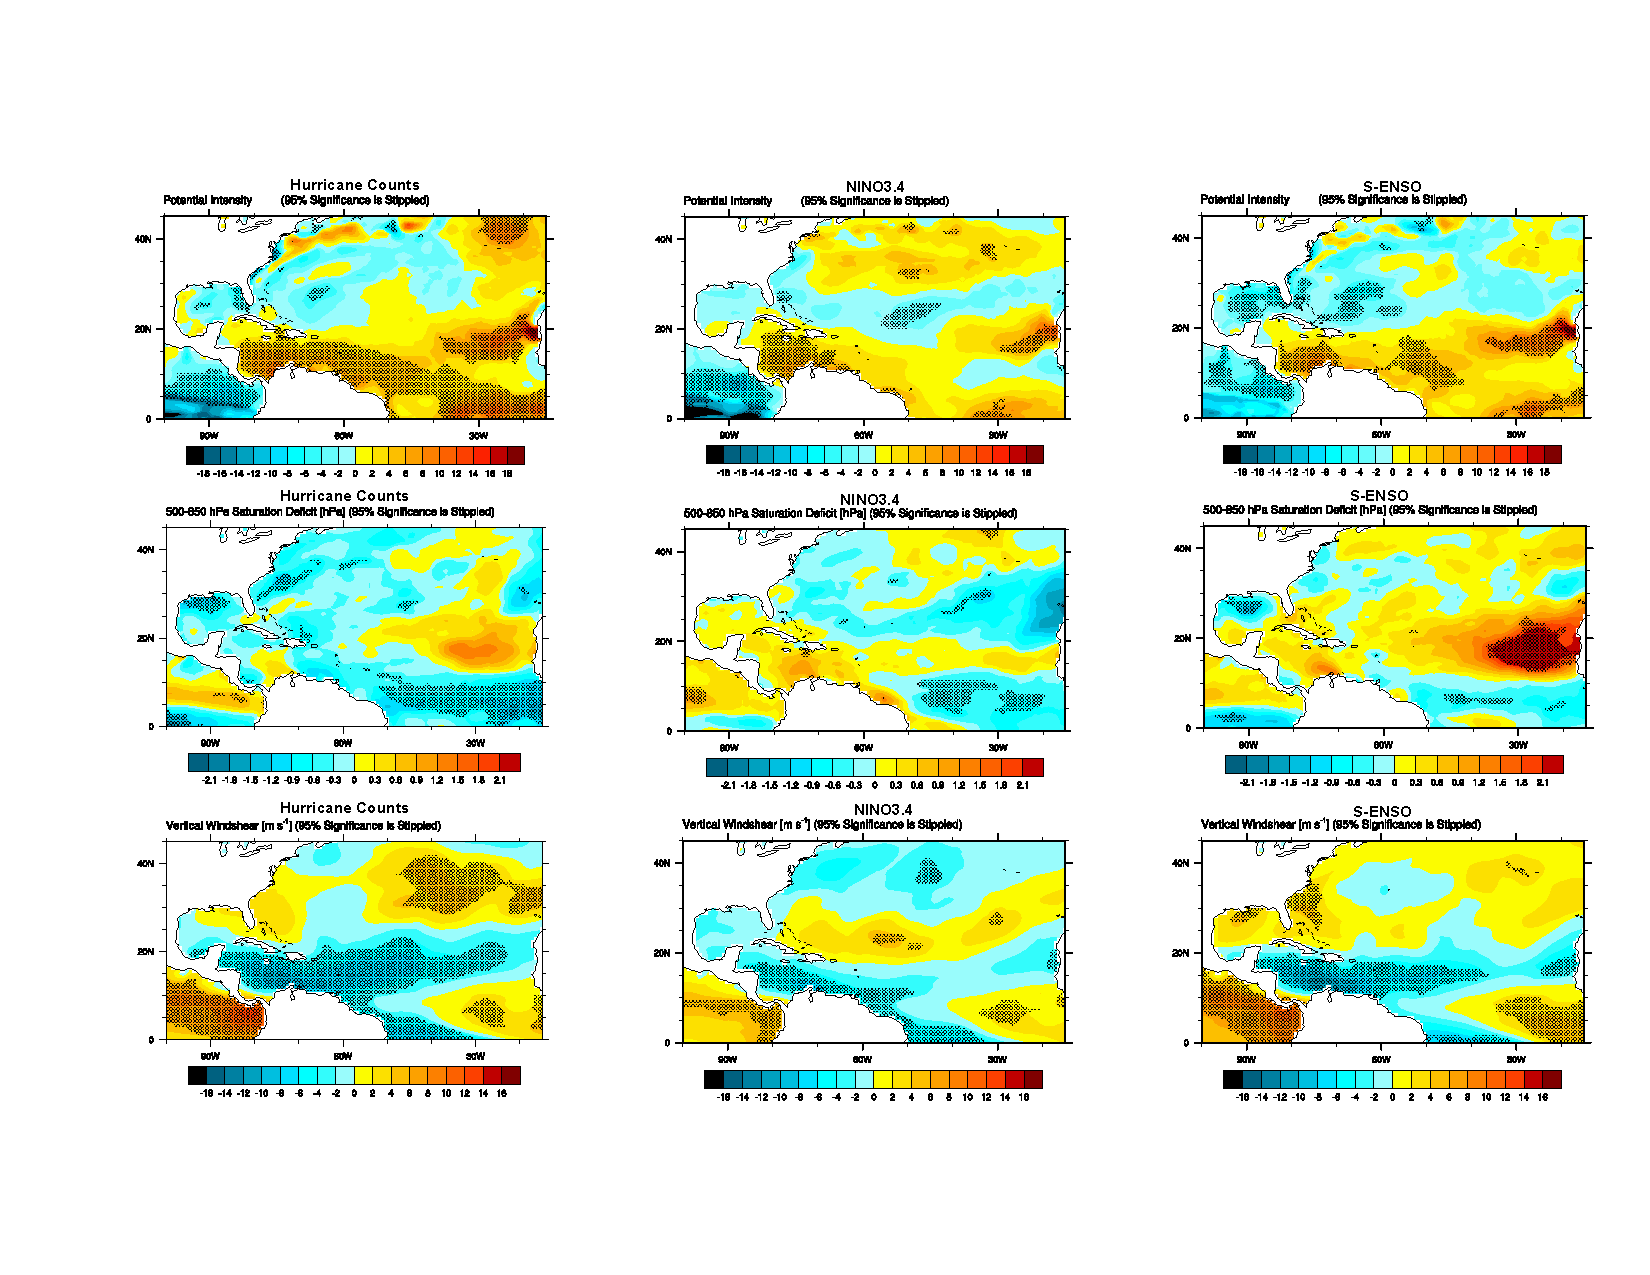
\includegraphics[width=7in]{figures/3_by_3_composites.pdf}
	\caption{composites for PI (top row), the difference in saturation deficit between 500 and 850 hPa (middle row), and vertical wind shear between 200 and 850 hPa (bottom) row. Each column shows the composites for hurricane counts (left), NINO3.4 (middle), and S-ENSO (right). $95\%$ significance intervals are shaded. Shaded area represents $95\%$ significance level. The hurricane count positive years (6) are: 1995, 2001, 2003, 2005, 2008, and 2010. The hurricane count negative years (8) are: 1982, 1983, 1986, 1987, 1992, 1993, 1994, 1997 and 2002. The NINO3.4 positive years (8) are: 1981, 1984, 1985, 1988, 1999, 2000, 2007, and 2008. The NINO3.4 negative years (6) are: 1982, 1987, 1991, 1992, 1997, 2002. S-ENSO positive years (6) are: 1989, 1995, 2003, 2005, 2008, 2010. S-ENSO negative years (6) are: 1982, 1983, 1991, 1997, 1998, 2002. For all three variables, S-ENSO reproduces the large scale environment over the Atlantic better than the traditional warming-based ENSO index NINO3.4}
	\label{fig:olr_comp}
\end{figure}